\documentclass[
11pt,notheorems,hyperref={pdfauthor=whatever}
]{beamer}
\usetheme[progressbar=frametitle]{metropolis}
\setbeamertemplate{headline}{
  \begin{beamercolorbox}[wd=\paperwidth,ht=2.5ex,dp=1.125ex]{}
  \end{beamercolorbox}
}
\input{loadslides.tex}

% Useful if not already loaded in loadslides.tex
\usepackage{amsmath, amssymb, bm}
\usepackage{tikz}
\usepackage{graphicx}
\usetikzlibrary{arrows.meta, positioning, matrix, calc}
\usetikzlibrary{matrix, positioning, arrows.meta}

\title[
Vaccination vs NPI]{Modeling the emergence of vaccine-resistant variants with Gaussian convolution}

\subtitle{COVID-19: Could the wrong strategy ruin vaccine efficiency?}

\author[
% Victor Schmit
]{
Victor Schmit, 
Cyprien Fievet,
Basma Zouine,
David Houri
}
\institute{CentraleSupélec}
\date{\today}

\begin{document}

{
\setbeamertemplate{footline}{}
\begin{frame}
	\titlepage
\end{frame}
}
\addtocounter{framenumber}{-1}

\begin{frame}{Part I: Article Approach : Optimal Control}
	\tableofcontents[part=1]
\end{frame}

\begin{frame}{Part II: A Reinforcement Learning Approach}
	\tableofcontents[part=2]
\end{frame}

\makepart{Vaccination vs NPI under variant evolution}

%------------------------------------------------
\section{Introduction}

\begin{frame}{Introduction}
	\begin{itemize}
		\item Vaccination reduces infection by the original strain.

		      \medskip

		\item But if infection remains high, vaccination may create a \alert{selection pressure}
		      toward more vaccine-resistant variants.

		      \medskip

		\item The paper asks:
	\end{itemize}

	\medskip

	\begin{block}{Question}
		\textbf{Is ``vaccinate as fast as possible'' always optimal, or can it backfire if NPIs are lifted too early ?}
	\end{block}
\end{frame}

% \begin{frame}{Key modeling idea}
% 	\begin{itemize}
% 		\item Variants are classified by two traits:
%
% 		      \medskip
%
% 		      \begin{itemize}
% 			      \item transmissibility,
%
% 			            \medskip
%
% 			      \item resistance to vaccine.
% 		      \end{itemize}
%
% 		      \medskip
%
% 		\item Instead of one infected compartment \(I(t)\), the model uses a matrix
% 		      \[
% 			      I(t)=\bigl(I_{ij}(t)\bigr)_{1\le i\le N,\;1\le j\le M}.
% 		      \]
%
% 		      \medskip
%
% 		\item Each entry \(I_{ij}(t)\) = fraction of population infected by variant \((i,j)\).
% 	\end{itemize}
% \end{frame}

%------------------------------------------------
\section{Compartments}\label{sec:model} % (fold)

\subsection{Variant space and compartments}

\begin{frame}{Variant grid}
	\begin{columns}[T]
		\column{0.52\textwidth}
		% \[
		% 	I(t)=
		% 	\begin{pmatrix}
		% 		I_{11}(t) & I_{12}(t) & \cdots & I_{1M}(t) \\
		% 		I_{21}(t) & I_{22}(t) & \cdots & I_{2M}(t) \\
		% 		\vdots    & \vdots    & \ddots & \vdots    \\
		% 		I_{N1}(t) & I_{N2}(t) & \cdots & I_{NM}(t)
		% 	\end{pmatrix}
		% \]

		\begin{itemize}
			\item Variants are classified by two traits:

			      \medskip

			      \begin{itemize}
				      \item transmissibility : $\beta_i$,

				            \medskip

				      \item resistance to vaccine : $\omega_j$.
			      \end{itemize}

			      \medskip

			\item Instead of one infected compartment \(I(t)\), the model uses a matrix
			      \[
				      I(t)=\bigl(I_{ij}(t)\bigr)_{1\le i\le N,\;1\le j\le M}.
			      \]

			      \medskip

			\item Each entry \(I_{ij}(t)\) = fraction of population infected by variant \((i,j)\).
		\end{itemize}


		\column{0.48\textwidth}
		\begin{center}
			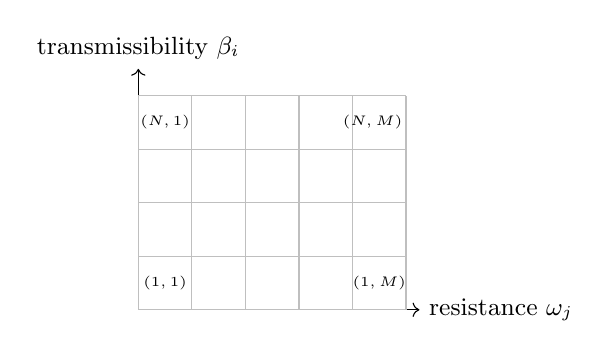
\begin{tikzpicture}[scale=0.85]
				\draw[->] (0,0) -- (4.2,0) node[right] {\small resistance \(\omega_j\)};
				\draw[->] (0,0) -- (0,3.6) node[above] {\small transmissibility \(\beta_i\)};
				\draw[step=0.8, gray!50] (0,0) grid (4,3.2);
				\node at (0.4,0.4) {\tiny \((1,1)\)};
				\node at (3.6,0.4) {\tiny \((1,M)\)};
				\node at (0.4,2.8) {\tiny \((N,1)\)};
				\node at (3.5,2.8) {\tiny \((N,M)\)};
			\end{tikzpicture}
		\end{center}

		\[
			\omega_j=\frac{j-1}{M-1},
			\qquad
			\beta_i \text{ increasing with } i
		\]
	\end{columns}
\end{frame}

% \begin{frame}{Compartments}
% 	\[
% 		S(t),\quad V(t),\quad I(t)=\bigl(I_{ij}(t)\bigr),\quad R(t)=\bigl(R_{ij}(t)\bigr),\quad D(t)
% 	\]
%
% 	\begin{itemize}
% 		\item \(S(t)\): susceptible
% 		\item \(V(t)\): vaccinated
% 		\item \(I_{ij}(t)\): infected by variant \((i,j)\)
% 		\item \(R_{ij}(t)\): recovered from variant \((i,j)\)
% 		\item \(D(t)\): deceased
% 	\end{itemize}
%
% 	\begin{block}{Remark}
% 		The matrix structure is what lets the model represent both
% 		\textbf{infectiousness} and \textbf{vaccine resistance} at the same time.
% 	\end{block}
% \end{frame}

%------------------------------------------------
\subsection{Compartment model}

\begin{frame}{Model Structure}
	\begin{columns}[T]
		\column{0.4\textwidth}
		\begin{itemize}
			\item \(n(t)\): vaccination rate
			\item \(\eta(t)\in(0,1]\): NPI coefficient
			      \begin{itemize}
				      \item \(\eta=1\): no restriction
				      \item smaller \(\eta\): stronger restrictions
			      \end{itemize}
			\item \(\mu\): fatality rate
			\item \(\gamma\): recovery rate
			\item \(\xi_{ijkl}\): reinfection tensor
			\item \(P\): mutation tensor
		\end{itemize}
		\column{0.5\textwidth}
		\begin{figure}
			\begin{center}
				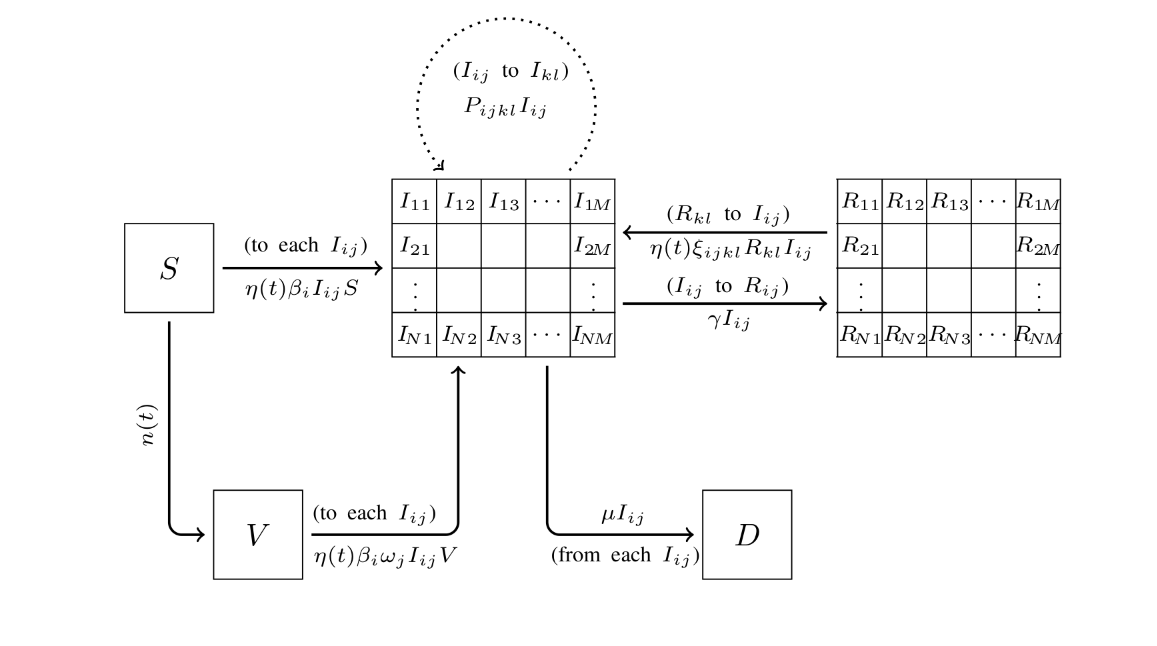
\includegraphics[width=1.\textwidth]{./figures/model.png}
			\end{center}
			\caption{Model Diagram : representation of state transitions}\label{fig:model}
		\end{figure}

	\end{columns}

\end{frame}

%------------------------------------------------
\subsection{Differential system}

\begin{frame}{Compact dynamical system}
	Using tensor notation, the model is
	\begin{align*}
		\frac{dS}{dt}(t)
		 & = -n(t)-\eta(t)\big[(\beta\otimes 1)\cdot\!\cdot I(t)\big]S(t)     \\[0.3em]
		\frac{dV}{dt}(t)
		 & = n(t)-\eta(t)\big[(\beta\otimes \omega)\cdot\!\cdot I(t)\big]V(t) \\[0.3em]
		\frac{dI}{dt}(t)
		 & = \eta(t)\big[(\beta\otimes 1)\circ I(t)\big]S(t)
		+ \eta(t)\big[(\beta\otimes \omega)\circ I(t)\big]V(t)                \\
		 & \quad -\mu I(t)-\gamma I(t)
		+ \eta(t)\big(\xi R(t)\big)\circ I(t)
		+ \Psi\big(P\cdot\!\cdot I(t)-I(t)\big)                               \\[0.3em]
		\frac{dR}{dt}(t)
		 & = \gamma I(t)-\eta(t)\big(\xi^{(3,4,1,2)}I(t)\big)\circ R(t)       \\[0.3em]
		\frac{dD}{dt}(t)
		 & = \mu I(t)\cdot\!\cdot(1\otimes 1)
	\end{align*}
\end{frame}

% \begin{frame}{Entrywise interpretation for \(I_{ij}\)}
% 	For one variant \((i,j)\), the infected dynamics combine:
% 	\begin{itemize}
% 		\item infections from susceptibles,
% 		\item infections from vaccinated people,
% 		\item deaths and recoveries,
% 		\item reinfection from recovered people,
% 		\item mutation inflow/outflow from neighboring variants.
% 	\end{itemize}
%
% 	\vspace{0.4em}
% 	Schematically:
% 	\[
% 		\frac{dI_{ij}}{dt}
% 		=
% 		\underbrace{\eta \beta_i I_{ij} S}_{S\to I_{ij}}
% 		+
% 		\underbrace{\eta \beta_i \omega_j I_{ij} V}_{V\to I_{ij}}
% 		-
% 		\underbrace{(\mu+\gamma)I_{ij}}_{\text{exit}}
% 		+
% 		\underbrace{\text{reinfection}}_{\xi}
% 		+
% 		\underbrace{\text{mutation}}_{P,\Psi}
% 	\]
% \end{frame}

%------------------------------------------------
\subsection{Mutation and reinfection}

\begin{frame}{Gaussian mutation operator}

	Schematically:
	\[
		\frac{dI_{ij}}{dt}
		=
		\underbrace{\eta \beta_i I_{ij} S}_{S\to I_{ij}}
		+
		\underbrace{\eta \beta_i \omega_j I_{ij} V}_{V\to I_{ij}}
		-
		\underbrace{(\mu+\gamma)I_{ij}}_{\text{exit}}
		+
		\underbrace{\text{reinfection}}_{\xi}
		+
		\underbrace{\text{mutation}}_{P,\Psi}
	\]

	Mutation is modeled as a Gaussian blur on the matrix \(I\) with a cutoff (to prevent the emergence of dangerous variant at the very beginning).

	\[
		G_\sigma(t)=\frac{1}{\sqrt{2\pi}\sigma}\exp\!\left(-\frac{t^2}{2\sigma^2}\right)
	\]

	% For each cell \((i,j)\),
	% \[
	% 	(P\cdot\!\cdot I)_{ij}
	% 	=
	% 	\sum_{k=1}^{N}\sum_{l=1}^{M}
	% 	G_\sigma(i-k)\,G_\sigma(j-l)\,I_{kl}.
	% \]

\end{frame}

% \begin{frame}{Reinfection tensor}
% 	Recovered individuals from variant \((k,l)\) may be reinfected by \((i,j)\) through
% 	\[
% 		\xi_{ijkl}.
% 	\]
%
% 	The paper imposes
% 	\[
% 		\xi_{ijij}=0
% 	\]
% 	and chooses
% 	\[
% 		\xi_{ijkl}=\frac{C}{M}\,[\omega_l-\omega_j]_+.
% 	\]
%
% 	\begin{block}{Interpretation}
% 		Reinfection is easier when the new variant is more vaccine-resistant / immune-escaping
% 		than the one previously encountered.
% 	\end{block}
% \end{frame}

%------------------------------------------------


%------------------------------------------------
\section{Optimal control}

\begin{frame}{Optimal control problem}
	Controls:
	\[
		u(t)=(n(t),\eta(t)).
	\]

	Constraints:
	\[
		\sup_{t\in[0,T]} n(t)\le n_{\mathrm{SUP}},
		\qquad
		\inf_{t\in[0,T]} \eta(t)\ge \eta_{\mathrm{INF}}.
	\]

	Cost to minimize:
	\[
		D(T)=\mu\int_0^T I(t)\cdot\!\cdot(1\otimes 1)\,dt.
	\]

	\begin{block}{Interpretation}
		Choose the vaccination intensity and NPI level to minimize mortality.
	\end{block}
\end{frame}

\begin{frame}{Hamiltonian}
	State:
	\[
		x(t)=\bigl(S(t),I(t),R(t),V(t)\bigr),
		\qquad
		p(t)=\bigl(p_S(t),p_I(t),p_R(t),p_V(t)\bigr).
	\]

	Hamiltonian:
	\[
		H(x,u,p)
		=
		\mu I\cdot\!\cdot(1\otimes 1)
		+
		p_S\frac{\partial S}{\partial t}
		+
		p_I\cdot\!\cdot\frac{\partial I}{\partial t}
		+
		p_R\cdot\!\cdot\frac{\partial R}{\partial t}
		+
		p_V\frac{\partial V}{\partial t}.
	\]

	Pontryagin condition:
	\[
		\frac{\partial p}{\partial t}(t)=-\nabla_x H(x(t),u(t),p(t)),
		\qquad
		p(T)=0.
	\]
\end{frame}

\begin{frame}{Switching functions}
	Differentiating the Hamiltonian with respect to controls gives:
	\[
		\Lambda_n(t)=\frac{\partial H}{\partial n}=p_V-p_S
	\]

	and
	\begin{align*}
		\Lambda_\eta(t)=\frac{\partial H}{\partial \eta}
		 & =
		-p_S\big((\beta\otimes 1)\cdot\!\cdot I(t)\big)S(t)
		-p_V\big((\beta\otimes \omega)\cdot\!\cdot I(t)\big)V(t) \\
		 & \quad
		-p_R\cdot\!\cdot\big(\xi^{(3,4,1,2)}I(t)\circ R(t)\big)  \\
		 & \quad
		+p_I\cdot\!\cdot
		\Big(
		((\beta\otimes 1)\circ I(t))S
		+
		((\beta\otimes \omega)\circ I(t))V
		+
		\xi R(t)\circ I(t)
		\Big).
	\end{align*}
\end{frame}

\begin{frame}{Bang-bang structure and control square}
	A necessary optimality condition is:
	\[
		u^*(t)\in
		(\{0,n_{\mathrm{SUP}}\}\times[\eta_{\mathrm{INF}},1])
		\cup
		([0,n_{\mathrm{SUP}}]\times\{\eta_{\mathrm{INF}},1\}).
	\]
	\begin{figure}
		\begin{center}
			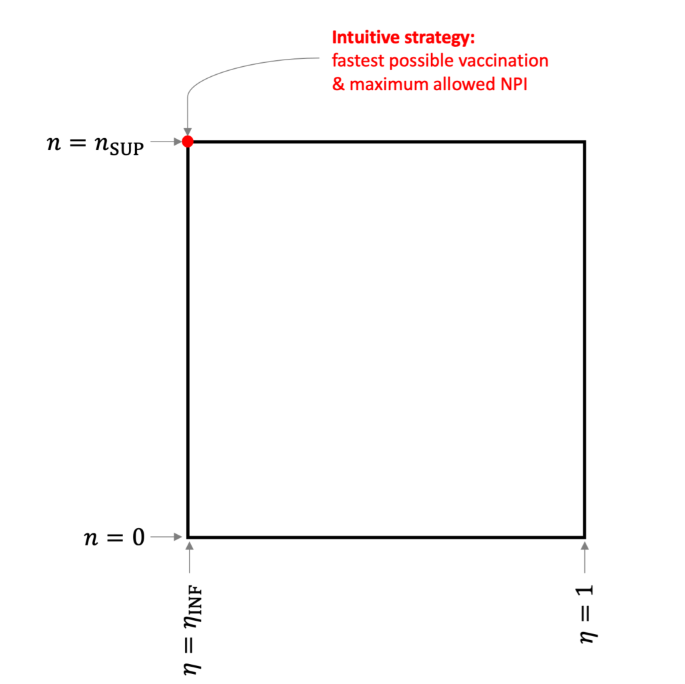
\includegraphics[width=0.35\textwidth]{figures/bang.png}
		\end{center}
		\caption{Bang-bang control : induced geometry of the solution}\label{fig:bang}
	\end{figure}


\end{frame}

\begin{frame}{How the paper computes the optimum}
	\textbf{Method 1: adjoint-based iteration}
	\begin{itemize}
		\item start from the intuitive policy;
		\item compute the adjoint state;
		\item update the controls using the signs of \(\Lambda_n\) and \(\Lambda_\eta\);
		\item smooth the updates with a relaxation parameter.
	\end{itemize}

	\textbf{Method 2: simulated annealing}
	\begin{itemize}
		\item discretize the control square;
		\item search for a near-optimal switching policy.
	\end{itemize}
\end{frame}

%------------------------------------------------
\section{Results and interpretation}

\begin{frame}{Simulation scenarios}
	Three scenarios are simulated:
	\begin{enumerate}
		\item low infection, no NPI;
		\item high infection, no NPI;
		\item high infection, with NPI initially.
	\end{enumerate}

	Typical parameters:
	\[
		N=30,\qquad M=40,\qquad R_0^{\max}=15,\qquad \gamma=0.09,\qquad \mu=0.02.
	\]

	\[
		n=0.006\quad \text{(0.6\% of the population vaccinated per day)}
	\]

	\begin{block}{Qualitative result}
		Vaccination works in low prevalence, and in high prevalence only if NPIs are maintained at least initially.
	\end{block}
\end{frame}

\begin{frame}{Main simulation insight}
	\begin{itemize}
		\item High infection + vaccination + no NPI:

		      % \medskip

		      \begin{itemize}
			      \item the original strain is reduced,

			            \medskip

			      \item but resistant variants are selected,

			            \medskip

			      \item a second peak appears.
		      \end{itemize}

		      \medskip

		\item High infection + vaccination + initial NPI:

		      % \medskip

		      \begin{itemize}
			      \item variants do not get enough time to emerge,

			            \medskip

			      \item pandemic is controlled.
		      \end{itemize}
	\end{itemize}
\end{frame}

\begin{frame}{Counterintuitive result}
	\begin{itemize}
		\item In the high-infection / no-NPI scenario, the intuitive strategy is \alert{not optimal}.
		\item The near-optimal strategy delays vaccination to limit selection of highly resistant variants.
		\item This still has a large death toll, but lower than the naive fast-vaccination policy without NPIs.
	\end{itemize}

	\begin{block}{Message}
		The short-term best action is not always the long-term best action when evolution is present.
	\end{block}
\end{frame}

\begin{frame}{Takeaways}
	\begin{itemize}
		\item The core novelty is replacing the scalar infected compartment by the matrix \(I_{ij}\).
		\item Mutation is modeled by Gaussian convolution in variant space.
		\item The optimal control problem is solved with Pontryagin + numerical search.
		\item Vaccination and NPIs must be analyzed jointly because they shape \textbf{selection pressure}.
	\end{itemize}
\end{frame}

\begin{frame}{Limitations}
	\begin{itemize}
		\item qualitative rather than predictive model;
		\item no waning immunity;
		\item one vaccine type only;
		\item mutation operator is phenomenological;
		\item no age / space / asymptomatic structure.
	\end{itemize}
\end{frame}

\makepart{Other approaches}

%--------------------------------------------------
\begin{frame}{RL Control (2D)}
	\begin{itemize}
		\item Control both:
		      \begin{itemize}
			      \item Vaccination rate $n_t$
			      \item NPI intensity $\eta_t$
		      \end{itemize}
		\item State = epidemic + variant distribution
		\item Goal: minimize infections, deaths, and evolution
	\end{itemize}

	\begin{figure}
		\begin{center}
			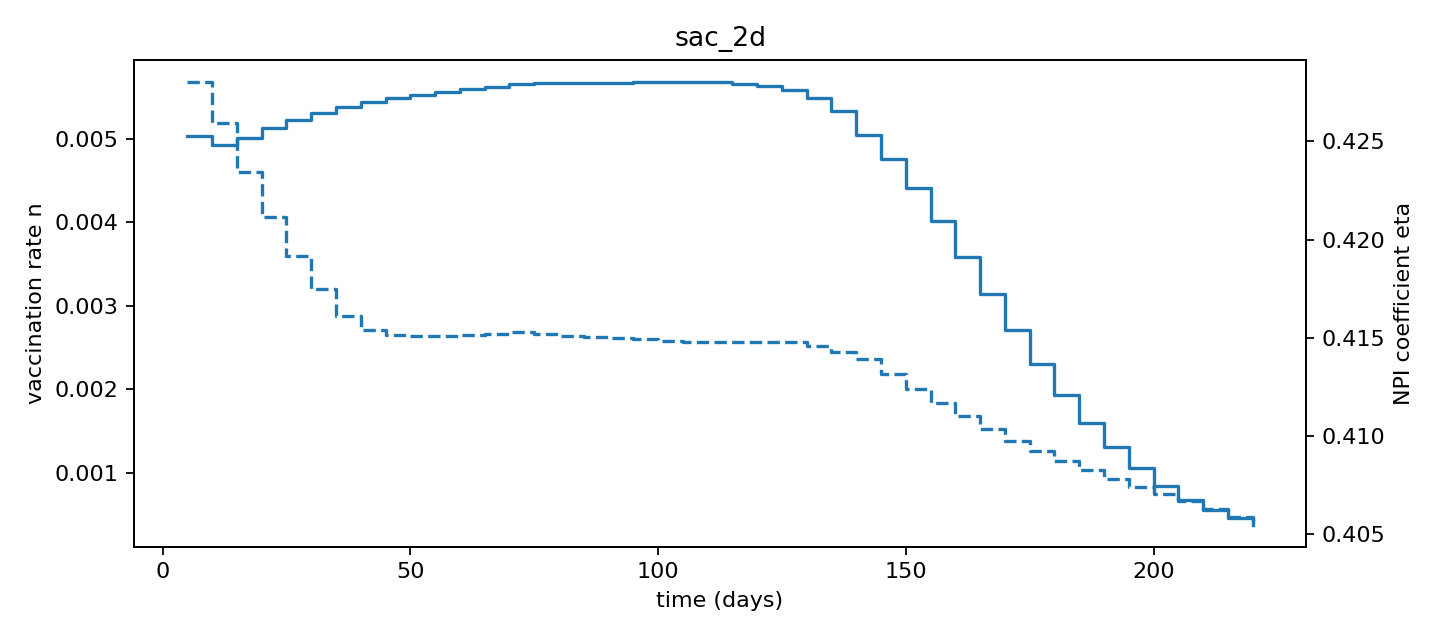
\includegraphics[width=0.65\textwidth]{./figures/sac_2d_controls.png}
		\end{center}
		\caption{}\label{fig:}
	\end{figure}
\end{frame}

%--------------------------------------------------
\begin{frame}{Algorithm (SAC)}
	\begin{columns}[T]
		\column{0.47\textwidth}
		\begin{itemize}
			\item Continuous control (no discrete policies)
			\item Learns policy $\pi(a|s)$
			\item Balances:
			      \begin{itemize}
				      \item epidemic suppression
				      \item evolutionary pressure
			      \end{itemize}
		\end{itemize}

		\column{0.5\textwidth}
		\begin{figure}
			\begin{center}
				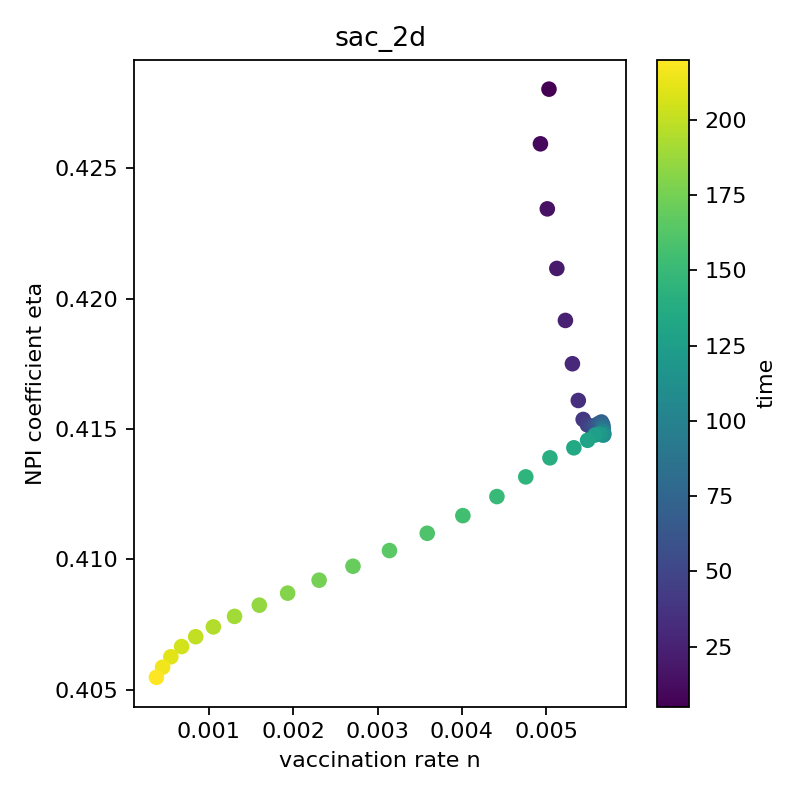
\includegraphics[width=0.75\textwidth]{./figures/sac_2d_phase_controls.png}
			\end{center}
			\caption{}\label{fig:}
		\end{figure}

	\end{columns}

\end{frame}

%--------------------------------------------------
\begin{frame}{Baseline: No Control}
	\begin{itemize}
		\item Large outbreak
		\item No strong evolution
	\end{itemize}

	\begin{center}
		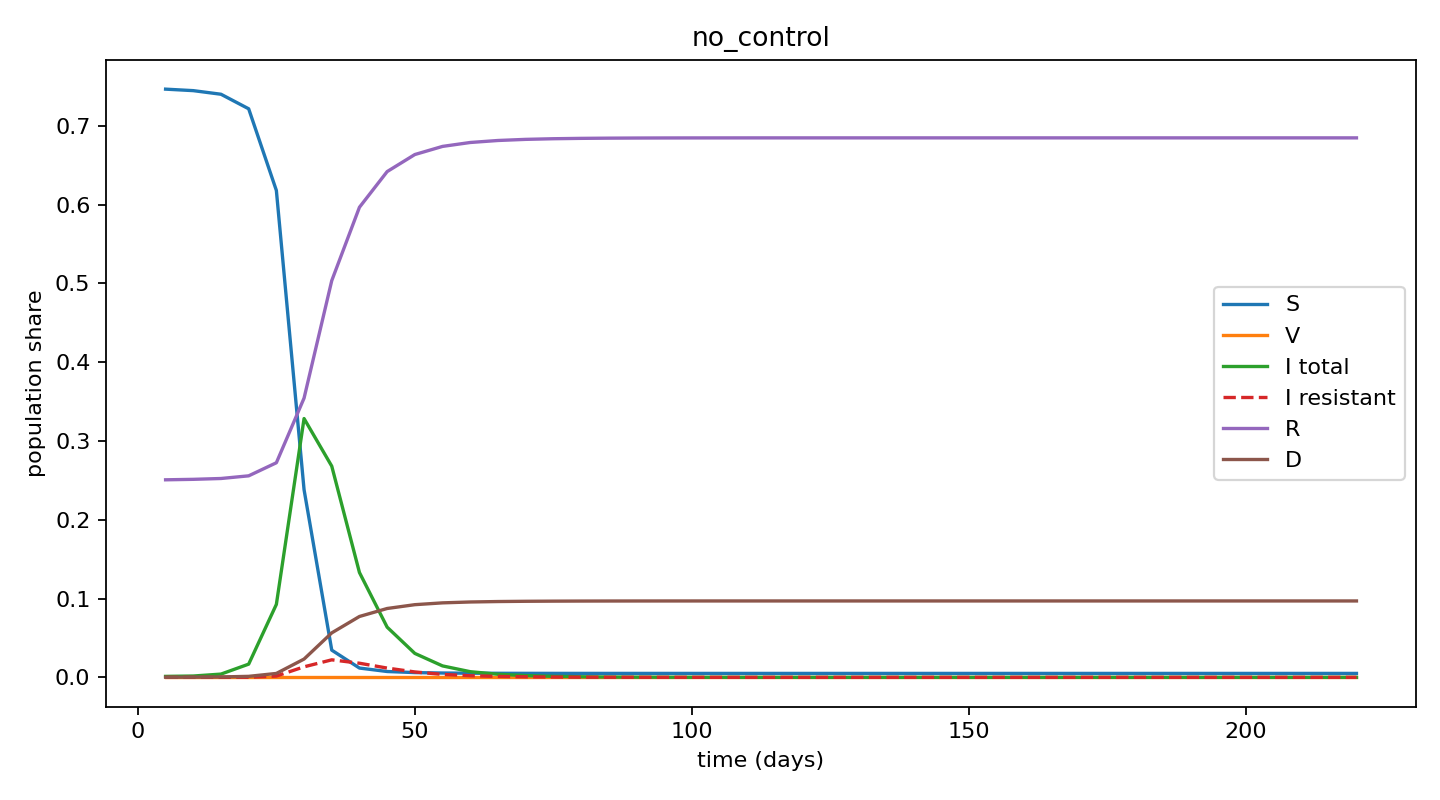
\includegraphics[width=0.45\linewidth]{./figures/no_control_compartments.png}
		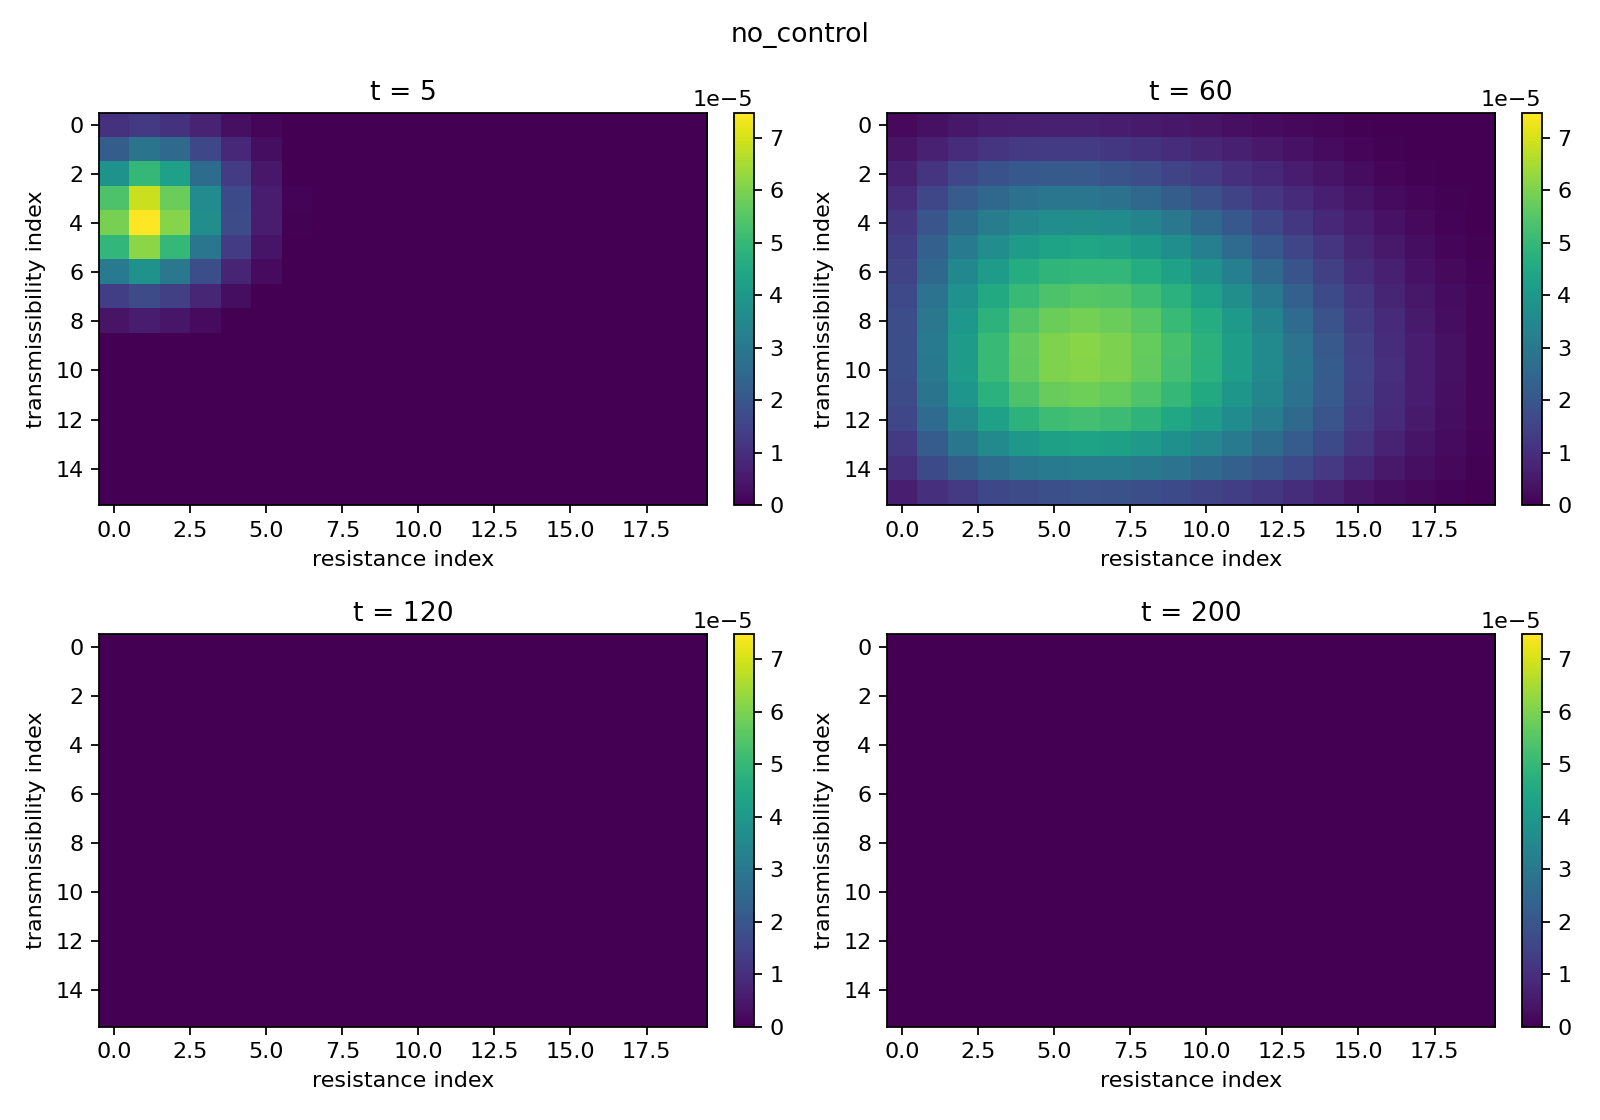
\includegraphics[width=0.45\linewidth]{./figures/no_control_variants.png}
	\end{center}
\end{frame}

%--------------------------------------------------
\begin{frame}{Baseline: Vaccination Only}
	\begin{itemize}
		\item Lower peak infection
		\item Higher deaths (!)
		\item Resistance emerges
	\end{itemize}

	\begin{center}
		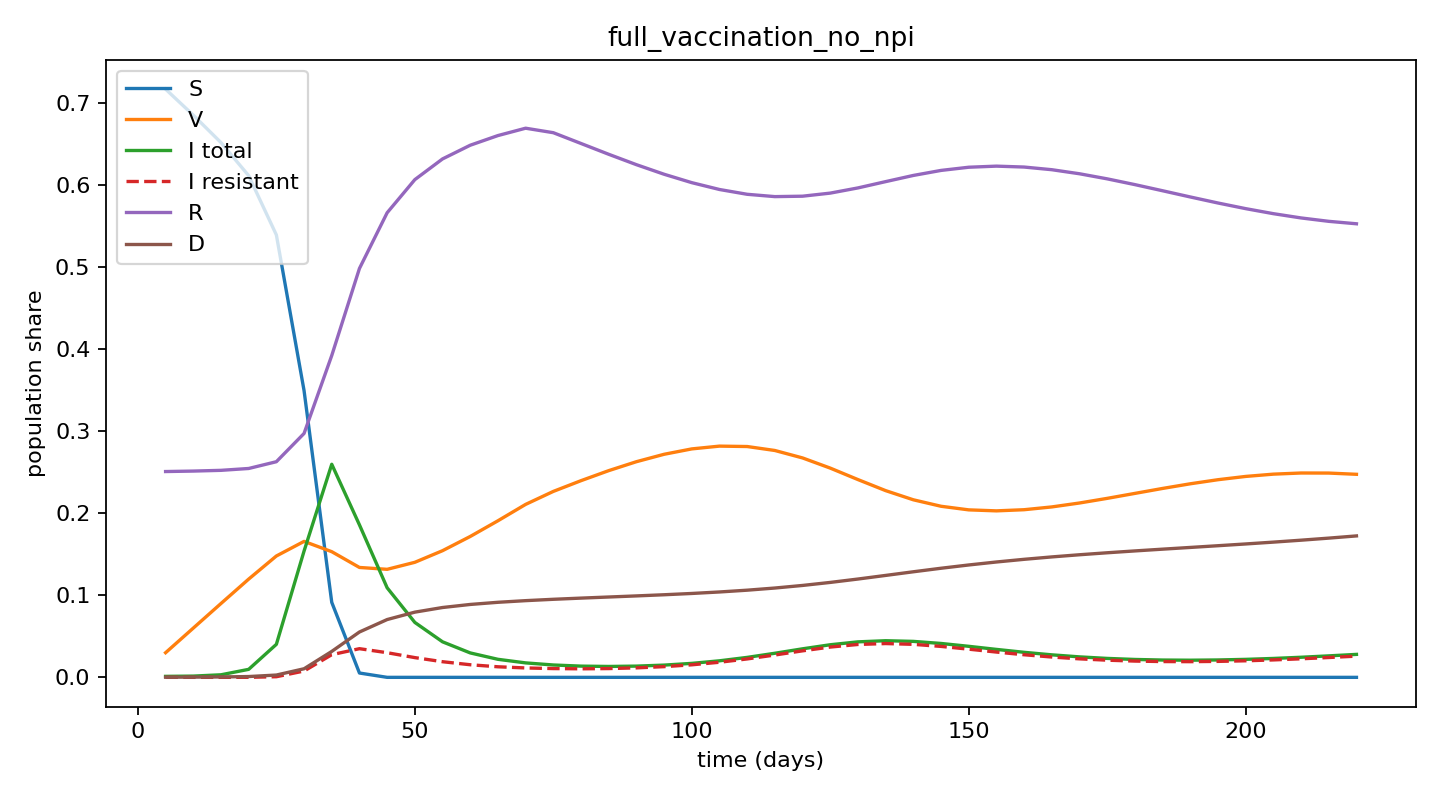
\includegraphics[width=0.45\linewidth]{./figures/full_vaccination_no_npi_compartments.png}
		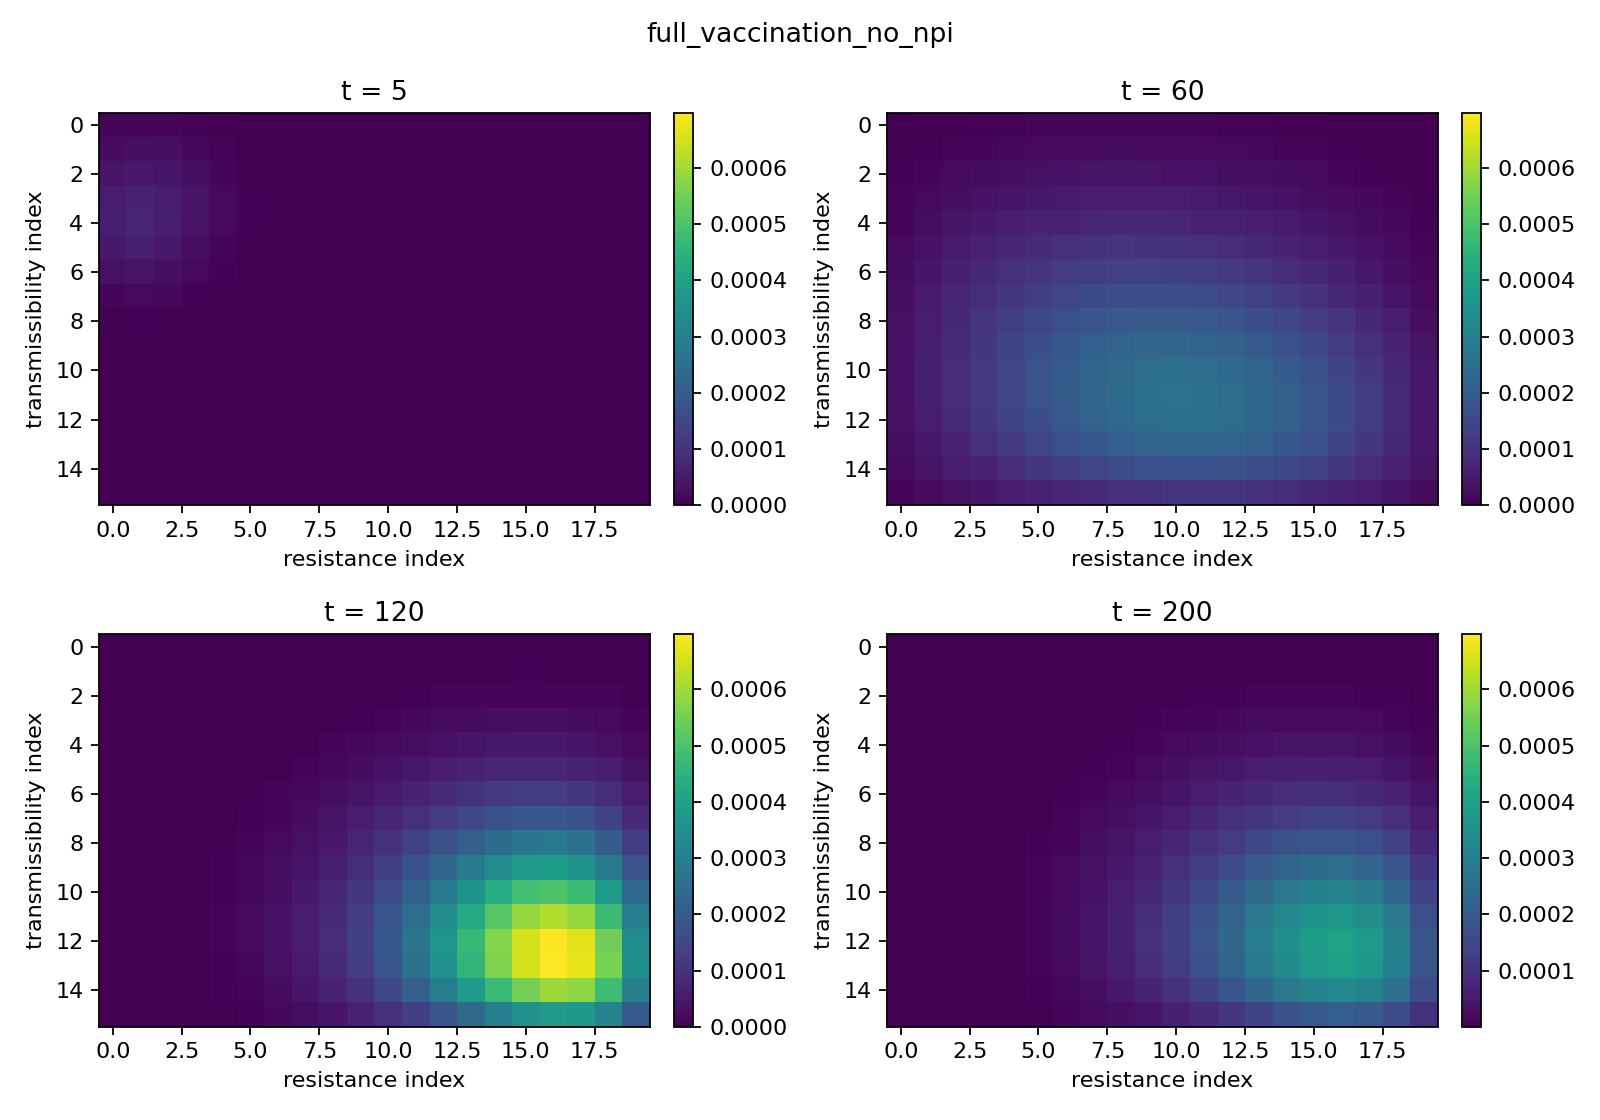
\includegraphics[width=0.45\linewidth]{./figures/full_vaccination_no_npi_variants.png}
	\end{center}
\end{frame}

%--------------------------------------------------
\begin{frame}{Baseline: Vaccination + NPI}
	\begin{itemize}
		\item Even lower infection
		\item Strong evolutionary pressure
		\item High resistance + transmissibility
	\end{itemize}

	\begin{center}
		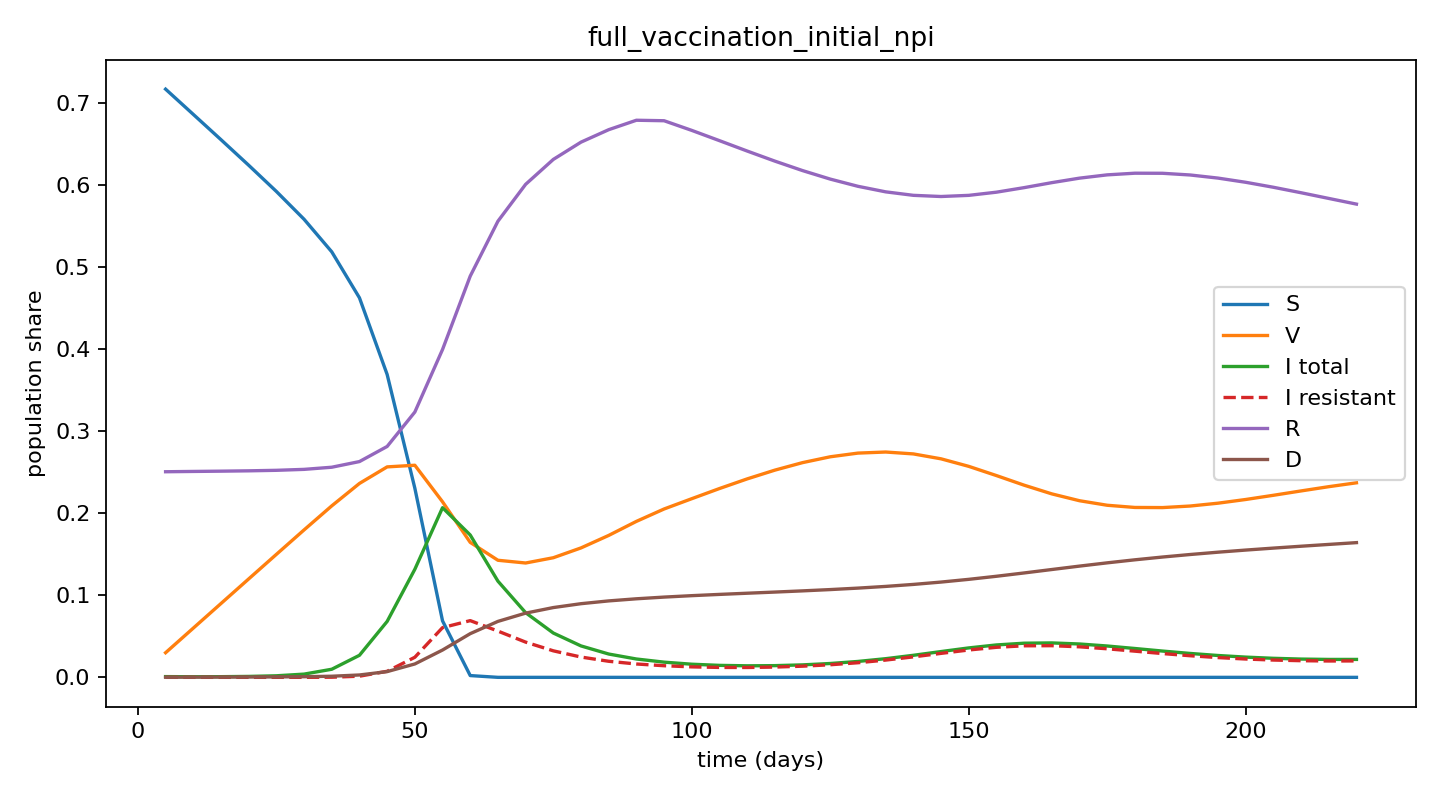
\includegraphics[width=0.45\linewidth]{./figures/full_vaccination_initial_npi_compartments.png}
		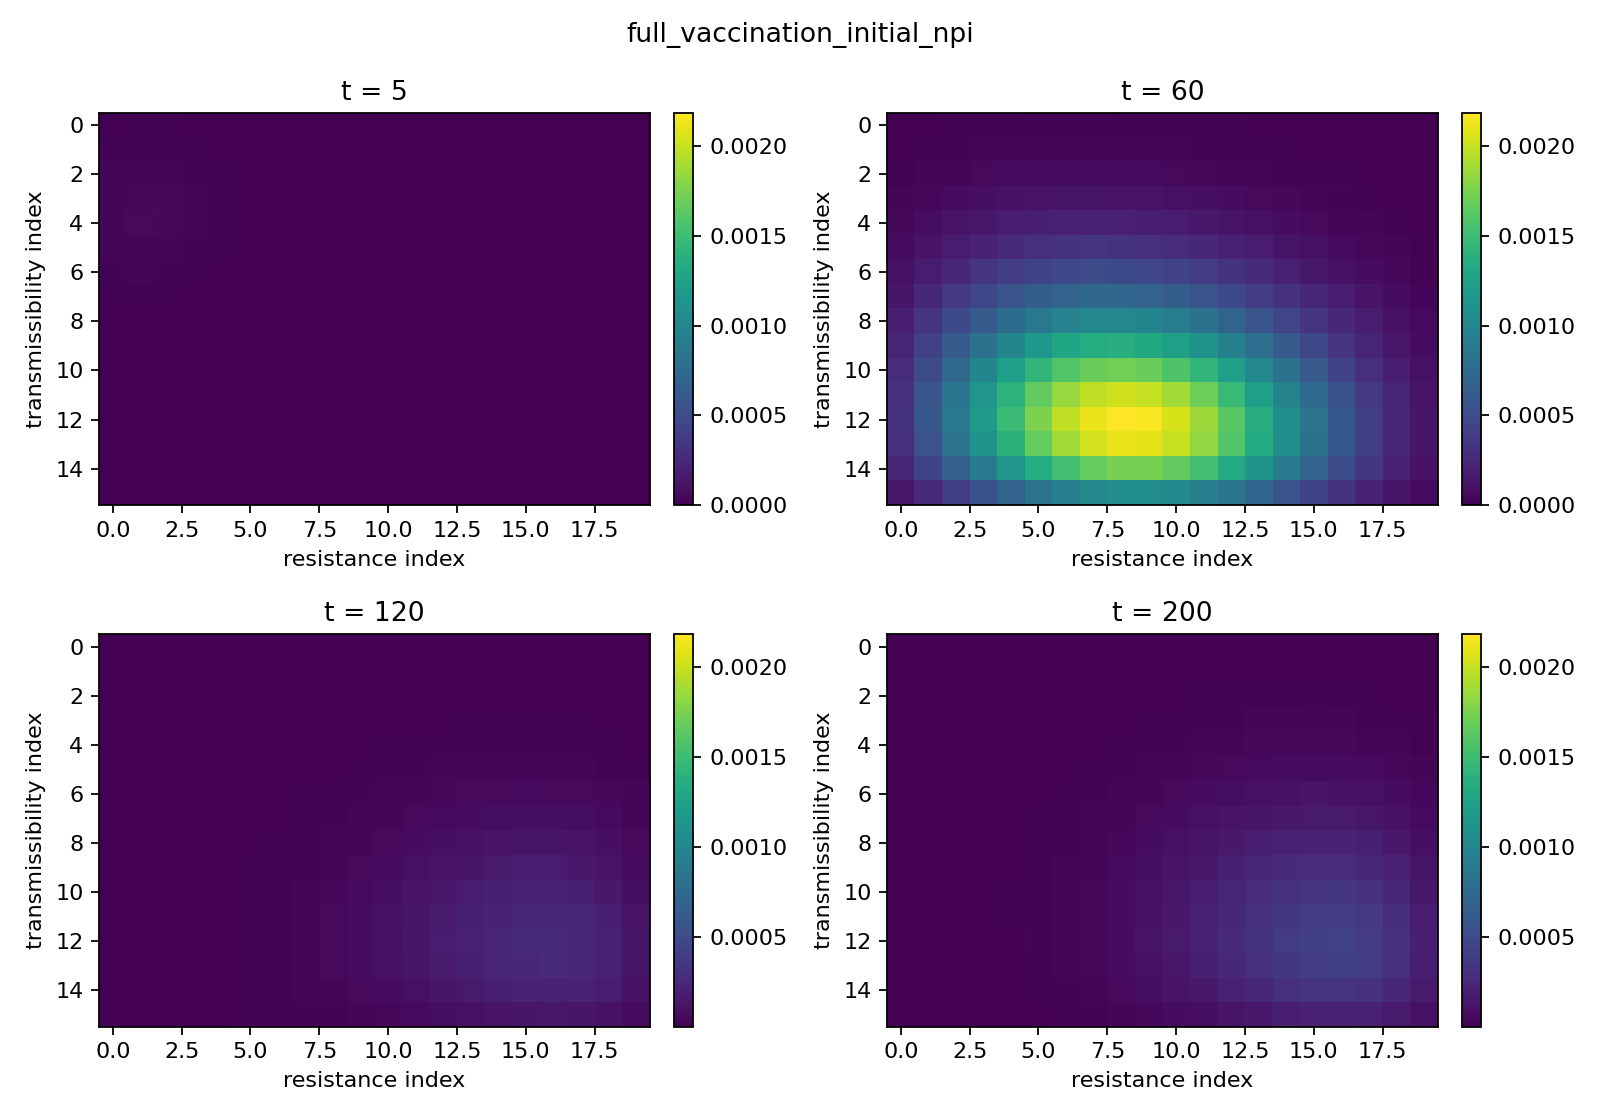
\includegraphics[width=0.45\linewidth]{./figures/full_vaccination_initial_npi_variants.png}
	\end{center}
\end{frame}

%--------------------------------------------------
\begin{frame}{Delayed Vaccination}
	\begin{itemize}
		\item Two waves
		\item Highest resistance
	\end{itemize}

	\begin{center}
		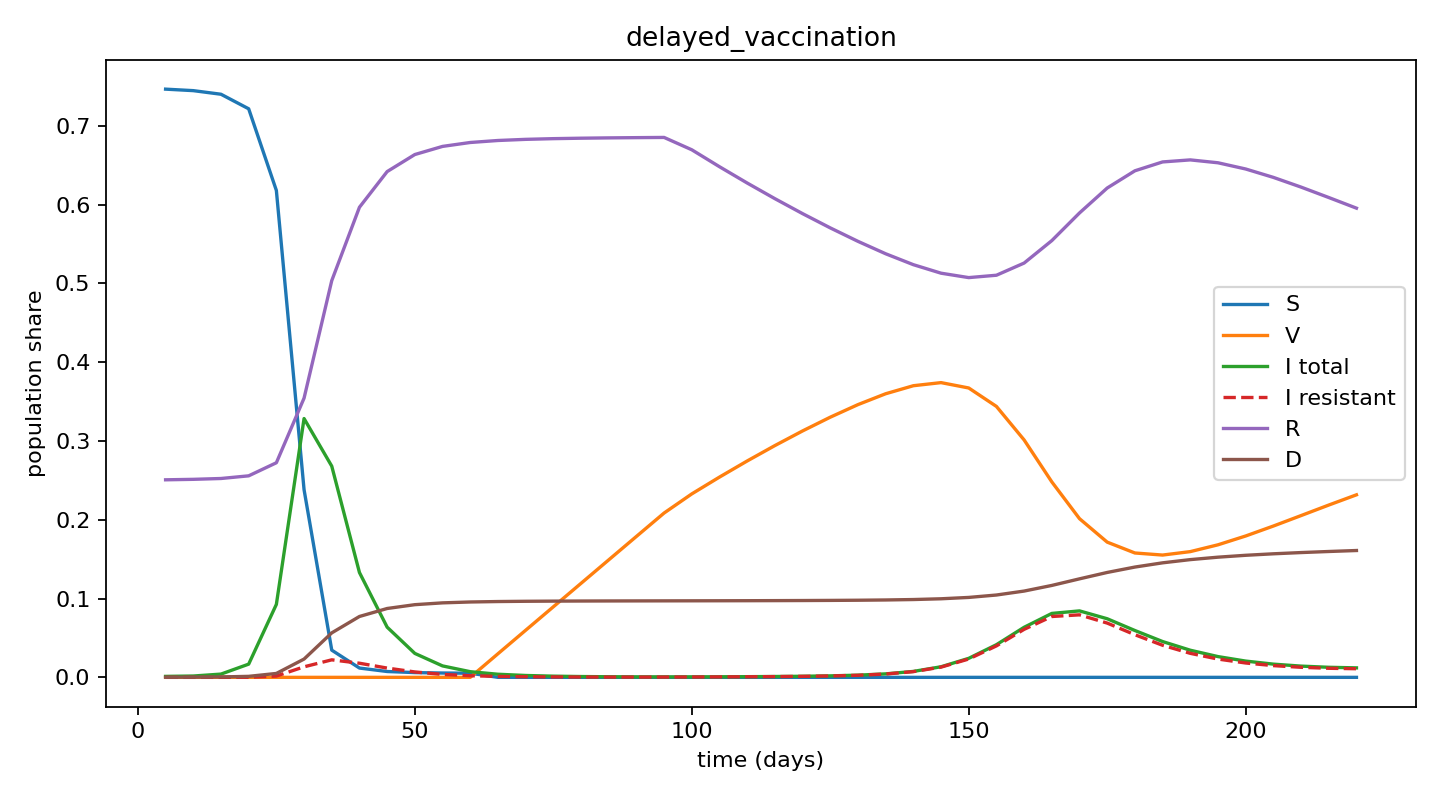
\includegraphics[width=0.45\linewidth]{./figures/delayed_vaccination_compartments.png}
		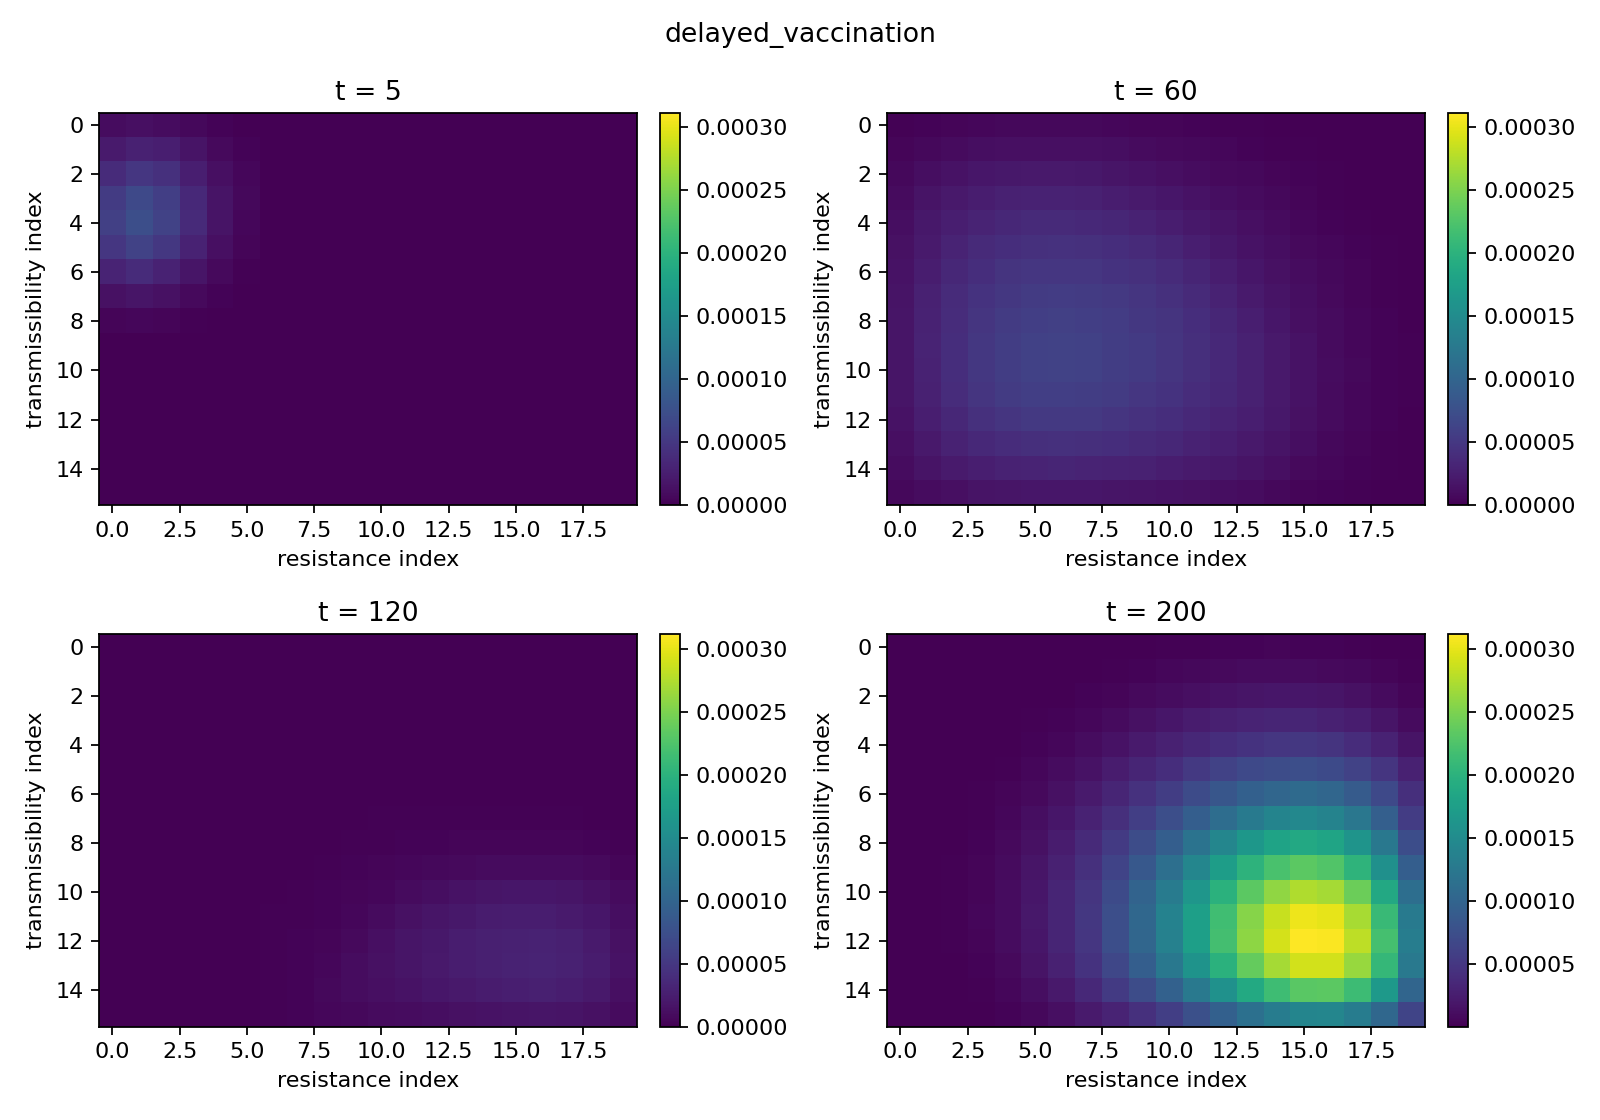
\includegraphics[width=0.45\linewidth]{./figures/delayed_vaccination_variants.png}
	\end{center}
\end{frame}

%--------------------------------------------------
\begin{frame}{RL (SAC 2D) Results}
	\begin{itemize}
		\item No large outbreak
		\item Near-zero deaths
		\item No resistant variants
	\end{itemize}

	\begin{center}
		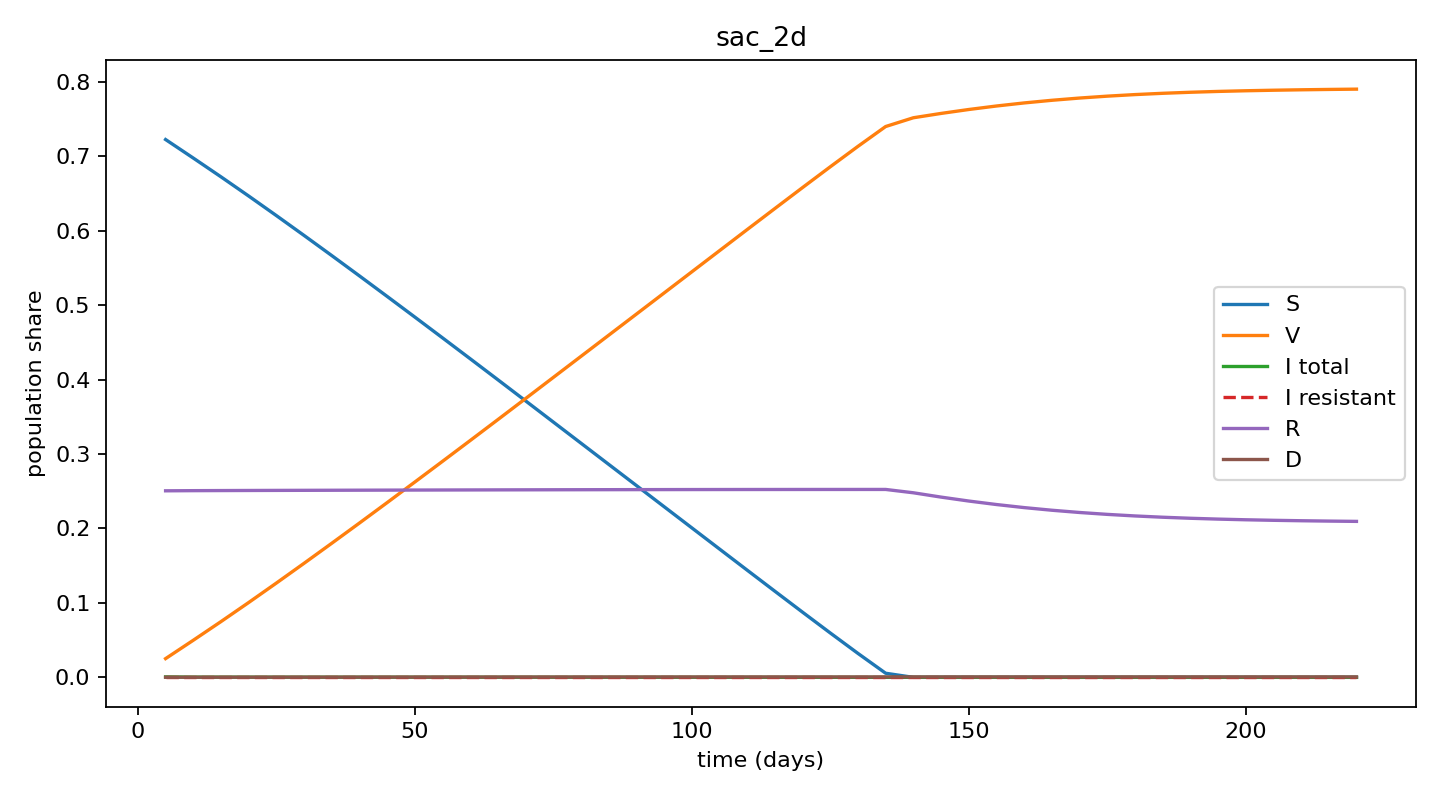
\includegraphics[width=0.45\linewidth]{./figures/sac_2d_compartments.png}
		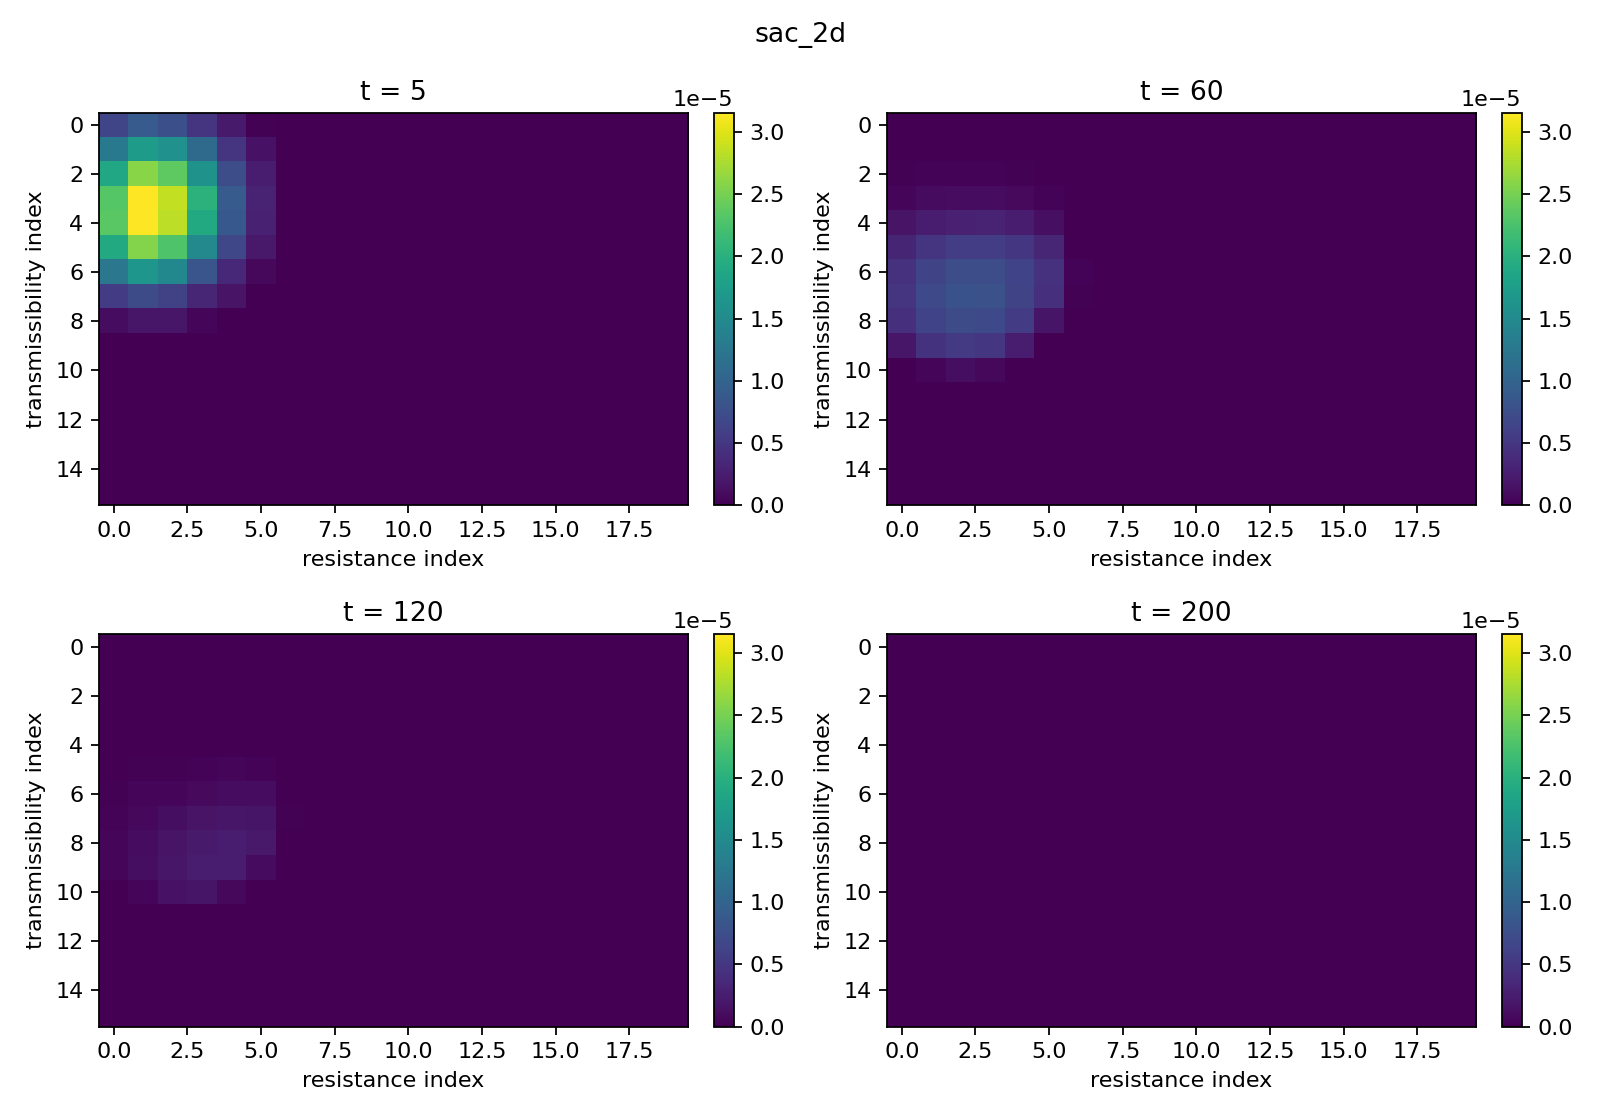
\includegraphics[width=0.45\linewidth]{./figures/sac_2d_variants.png}
	\end{center}
\end{frame}

%--------------------------------------------------
\begin{frame}{Key Insight}
	\begin{itemize}
		\item Strong static control $\Rightarrow$ strong evolution
		\item Weak control $\Rightarrow$ large outbreak
		\item RL $\Rightarrow$ balance both
	\end{itemize}

	\begin{block}{Takeaway}
		Adaptive control prevents both epidemic spread and evolutionary escape
	\end{block}
\end{frame}

\end{document}
